%==============================================================================
% Section 3: DBR reduction protocol and route justification
%==============================================================================
\section{DBR reduction protocol and route justification}
\label{sec:dbr}

\subsection{The Dirac-before-Routh protocol}
\label{sec:dbr:protocol}

The phase space of the first-order EC+NY system consists of the tetrad, the
connection, and their conjugate momenta, and it carries many primary
constraints.  Our reduction procedure adopts the following order \emph{as a
protocol}.

\begin{quote}
\textbf{DBR (Dirac-before-Routh) protocol.}
(i) Complete the Dirac--Bergmann algorithm~\cite{ref10,ref11,ref12}: generate
the secondary constraints from the consistency of the primary constraints, and
after closure classify first/second class and construct the Dirac bracket for
the second-class pairs.  (ii) Only then perform the Routh-type elimination /
reduction of the auxiliary variables (such as the non-dynamical connection
components) and present the reduced spectrum.
\end{quote}

DBR is not a new principle; it is the standard procedure of constrained
dynamics applied faithfully to this system.  The reverse order -- solving the
auxiliary connection variables by their field equations and substituting into
the action before the constraint analysis -- is called the \textbf{RBD
(Routh-before-Dirac)} route here.

\subsection{Why the order matters: a recognised issue}
\label{sec:dbr:order}

That substitution at the level of the action is not, in general, interchangeable
with substitution at the level of the equations of motion is an established
generality~\cite{ref13}.  Substitution is safe only for auxiliary variables
(whose own equations are algebraically solvable and free of derivatives);
otherwise a proof of equivalence is required.  In the Bianchi context it is also
classically known that the validity of imposing the symmetry at the level of the
action is restricted to class A (in class B it gives the wrong field
equations)~\cite{ref21,ref22}, and the equivalence of the Palatini and metric
formulations itself is a nontrivial statement to be proved by constraint
analysis~\cite{ref23}.  In adopting DBR as the standard, we select the order of
operations for which constraint equivalence is guaranteed against this known
``Palatini reduction non-commutativity'' (route dependence).

\subsection{Control experiment}
\label{sec:dbr:control}

To support the adoption of DBR empirically, we ran the RBD route as a
\textbf{control experiment}.  The verification was carried out in the Branch-A
scalar sector of the $\Sthree$ background.  The result is the following.

\begin{quote}
In the verified $\Sthree$ Branch-A scalar sector, eliminating the auxiliary
connection variables before the Dirac closure produces a Dirac-inequivalent
extra scalar mode.  The recomputation gives $N_{\rm phys}=0$ for
DBR\_KEEP\_ALL at all representative harmonic levels, whereas the spatial-$\omega$
and full-$K$ Routh variants give $N_{\rm phys}=1/1/2$ for $l=0,1,\ge2$.  At the
lowest harmonic level the comparison starts from the same Branch-A local
first-order Lagrangian, and reproduces the discrepancy DBR:0 / RBD:1 together
with $H_{PP}=-3/8<0$.  For $l\ge1$ the RBD extra count is treated as a
route-level gauge-breaking artefact; the negative-sign diagnostic is claimed
only at $l=0$ (scope details in Appendix~\ref{app:route}).
\end{quote}

This discrepancy is \emph{route-level}, not a physical instability.  We do not
draw from it any theorem that ``RBD is generally wrong.''  The claim is confined
to a single point: \emph{since route equivalence demonstrably fails in this
system, all subsequent physical topology claims are made within the DBR
protocol.}

\begin{table}[H]
\centering
\begingroup
\renewcommand{\arraystretch}{1.4}
\begin{tabularx}{\linewidth}{lLLl}
\toprule
Route & Order of closure and elimination & Outcome in $\Sthree$ Branch-A scalar sector & Status \\
\midrule
DBR & Dirac closure $\to$ Routh elimination &
$0$ physical scalars (kernel non-propagating; Section~\ref{sec:rankdefect}) &
\textbf{adopted} (standard) \\
RBD & Routh elimination $\to$ Dirac closure &
Dirac-inequivalent extra scalar mode ($H_{PP}=-3/8<0$ at $l=0$; route-level) &
control route (recorded) \\
\bottomrule
\end{tabularx}
\endgroup
\caption{Route taxonomy (compact version; details in
Appendix~\ref{app:route}).}
\label{tab:route}
\end{table}

\begin{figure}[H]
  \centering
  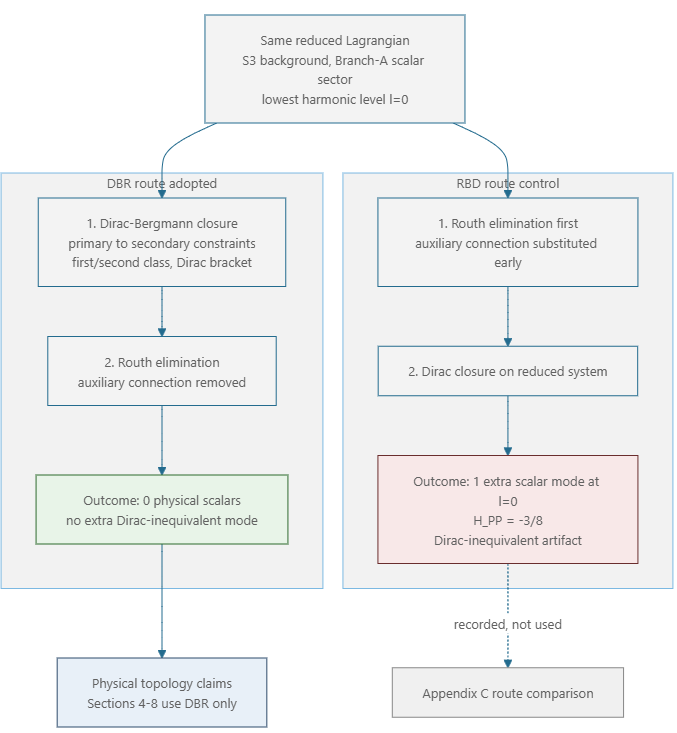
\includegraphics[width=0.95\textwidth]{figures/fig02_DBR-vs-RBD_route-comparison.png}
  \caption{DBR versus RBD route comparison.  From the same Branch-A local
    first-order Lagrangian, the two routes -- differing only in the order of
    operations -- are shown side by side.  DBR yields $0$ physical scalar
    degrees of freedom, while RBD gives a Dirac-inequivalent extra mode; at
    $l=0$ the diagnostic sign is $H_{PP}=-3/8<0$.  \emph{Scope}: the negative
    sign is claimed only for the lowest level; for $l\ge1$ the RBD extra count
    is recorded as a route-level gauge-breaking artefact.  The RBD outcome is
    not a physical instability.}
  \label{fig:route}
\end{figure}

\subsection{Scope declaration}
\label{sec:dbr:scope}

The claims of all subsequent sections
(Sections~\ref{sec:rankdefect}--\ref{sec:torsion}) are results under the DBR
protocol.  The RBD route is referred to only in the route-comparison details of
Appendix~\ref{app:route}.
